% To je predloga za poročila o domačih nalogah pri predmetih, katerih
% nosilec je Blaž Zupan. Seveda lahko tudi dodaš kakšen nov, zanimiv
% in uporaben element, ki ga v tej predlogi (še) ni. Več o LaTeX-u izveš na
% spletu, na primer na http://tobi.oetiker.ch/lshort/lshort.pdf.
%
% To predlogo lahko spremeniš v PDF dokument s pomočjo programa
% pdflatex, ki je del standardne instalacije LaTeX programov.

\documentclass[a4paper,11pt]{article}
\usepackage{a4wide}
\usepackage{fullpage}
\usepackage[utf8x]{inputenc}
\usepackage[slovene]{babel}
\selectlanguage{slovene}
\usepackage[toc,page]{appendix}
\usepackage[pdftex]{graphicx} % za slike
\usepackage{setspace}
\usepackage{color}
\definecolor{light-gray}{gray}{0.95}
\usepackage{listings} % za vključevanje kode
\usepackage{hyperref}
\renewcommand{\baselinestretch}{1.2} % za boljšo berljivost večji razmak
\renewcommand{\appendixpagename}{Priloge}
\renewcommand{\lstlistingname}{Koda}% Listing -> Algorithm
\usepackage{amsmath}
\usepackage{amssymb}
\definecolor{deepgreen}{rgb}{0,0.5,0}
\definecolor{deepblue}{rgb}{0,0,0.5}
\definecolor{ayu-comment}{RGB}{67,69,71}
\definecolor{ayu-bg}{RGB}{250,250,250}
\definecolor{ayu-accent}{RGB}{255, 153, 64}
\definecolor{ayu-func}{RGB}{57 ,158,	230}
\definecolor{ayu-string}{RGB}{134, 179, 0}

\lstset{ % nastavitve za izpis kode, sem lahko tudi kaj dodaš/spremeniš
language=Python,
basicstyle=\footnotesize,
basicstyle=\ttfamily\footnotesize\setstretch{1},
breaklines=true,
postbreak=\mbox{\textcolor{red}{$\hookrightarrow$}\space},
backgroundcolor=\color{ayu-bg},
emph={import,from,for,in,as,end,function},
emphstyle=\color{ayu-accent},
stringstyle=\color{ayu-string},
showstringspaces=false,
keywordstyle=\color{ayu-func},
commentstyle=\color{ayu-comment},
otherkeywords={read,getVars,optimize,write}
}

\title{Primerjava reševanja ILP v Matlab in Gurobi}
\author{David Rubin (david.rubin@student.um.si)}
\date{\today}

\begin{document}

\maketitle

\section{Uvod}

V tem poročilu si bomo ogledali kako se lahko pohitri reševanje ILP problemov z uvedbo distriburianega procesiranja. Kot standarden čas reševanja bomo uporabili MATLAB oziroma njegovo funkcijo \textit{intlinprog} iz \textit{optimization toolbox-a}.  Kot predlagano pohitritev, smo si v tem poročilu ogledali orodje Gurobi~\footnote{Orodje Gurobi je dostopno na \url{https://www.gurobi.com/}. Za potrebe te naloge smo uporabili akademsko licenco}. Orodje prav tako omogoča določevanje števila uporabljenih niti, tako da lahko orodje tudi nekoliko bolj pošteno primerjamo z \textit{intlinprog}, ko nastavimo enojno nit. Za testne probleme smo si izbrali zbirko MIPLIB2017~\cite{Miplib:2017}. Celotna zbirka je precej obsežna, zato smo se odločili za \textit{benchmark} verzijo, ki vključuje le del vseh problemov. Zbirko in pripravo testnih podatkov smo predstavili v poglavju~\ref{benchmark_data}. Predvidevamo, da je bralec seznanjen s programskim okoljem MATLAB, zato smo podali le kratek uvod v Gurobi.

\section{Gurobi}

Gurobi je komercialna programska oprema, ki omogoča optimiziranje problemov iz:
\begin{itemize}
\item lineranega programiranja (angl. \textit{linear programming} - LP),
\item mešanega celoštevilskega linearnega programiranja (angl. \textit{mixed-integer linear programming} - MILP),
\item kvadratičnega programiranja (angl. \textit{quadratic programming} - QP),
\item mešanega  celoštevilskega kvadratičnega programiranja (angl. \textit{mixed-integer quadratic programming} - MIQP),
\item kvadratično omejenega programiranja (angl. \textit{quadratically constrained programming} - QCP),
\item mešano celoštevilskega kvadratično omejenega programiranja (angl. \textit{Mixed-integer quadratically constrained programming} - MIQCP.
\end{itemize}
Pokriva torej veliko območje problemov, za zadnje štiri pa je vredno omeniti, da podpira tako konveksne kot tudi konkavne probleme. Za reševanje nabora problemov imajo implementirane metode Simplex in paralelno oviro s križanjem, sočasnostjo, in sejanjem (angl. \textit{parallel barrier with crossover, concurrent, and sifting}) za bolj zahtevne pa uporabijo tudi deterministično paralelno ne-tradicionalno iskanje, hevristike, rezanja ravnin in pa razbijanje simetrij~\cite{GurobiOptimizer:2020}. 	

Algoritmi so zasnovani deterministično, torej bi več zagonov skozi isti model dalo enake rezultate. Zasnovani so tudi tako, da po privzetem uporabijo vsa jedra, ki so v nekem sistemu na voljo. Trdijo tudi, da njihovi QCP in MIQCP algoritmi nudijo dvakrat boljšo učinkovitost kot njihov glavni tekmeci~\cite{GurobiBrochure:2020}. Slednje trditve ne moremo  sami potrditi, ne moremo pa je niti zavreči, tako da prepuščamo bralcu, da sam oceni resničnost. Podjetje so ustanovili dr. Robert Bixby, ki je pred tem tudi ustanovil CPLEX in pa Dr. Zonghao 	Gu ter Dr. Edward Rothberg. Slednja sta pred ustanovitvijo sodelovala pri CPLEX kot glavna inženirja~\cite{GurobiTeam:2020}. Kot zanimivost, ime \textit{GuRoBi} je nastalo iz njihovih priimkov. Med njihove partnerje spadajo podjetja kot je recimo Toyota, Microsoft, Google, AirFrance in pa tudi SAP.

Gurobi podpira množico programskih jezikov in oblik programiranja. Nudijo objektno orientirane vmesnike (\texttt{JAVA}, \texttt{C++}, \texttt{.NET} in \texttt{Python}), matrično orientiranie (\texttt{C}, \texttt{MATLAB} in \texttt{R}), povezavo do standardnih modelnih jezikov (\texttt{AIMMS}, \texttt{AMPL}, \texttt{MPL}) in druge~\cite{GurobiOptimizer:2020}. V kolikor bi orodje želeli uporabljati le v jeziku \texttt{Python} se lahko preskoči namestitev celotne knjižnice in uporabi \texttt{pip} ali \texttt{Anaconda} paket. Nudijo pa tudi možnost porazdeljenega reševanja problemov na gruči (\textit{Gurobi Remote Services}), ki pa zahteva ločeno licenco.

\subsection{Priprava okolja}
\label{gurobi_install}

Za uporabnike je na voljo vodič za hitro namestitev za vse tri večje operacijske sisteme\footnote{Vodič je dostopen na \url{https://www.gurobi.com/documentation/quickstart.html}}. Posebno pozornost je potrebno posvetiti sekciji za pridobitev akademske licence. Zahtevana je uporaba epoštnnega naslova univerze in imeti dostop do spleta v času aktivacije. Po prijavi nam je na voljo dostop do prenosa njihove knjižnice in CLI orodja\footnote{Programska oprema Gurobi se pridobi na naslovu \url{https://www.gurobi.com/downloads/gurobi-software/}}. Znotraj dokumenta navajajo, da se za akademski dostop poleg licenčnega ključa preverja tudi domensko ime iz lokacije dostopa. Pri naši aktivaciji se ni pojavila težava (ukaz \texttt{grbgetkey \textless koda\textgreater}), kljub temu, da smo med aktivacijo dostopali do njihovega strežnika zunaj omrežja univerze. V kolikor Gurobi med aktivacijo sporoči kakšno napako (primer \textit{hostname ... not recognized as belonging to an academic domain}), pa je možna uporaba VPN, ki je na voljo vsem študentom (in zaposlenim) Univerze v Mariboru.

V kolikor je orodje nameščeno in je bila aktivacija uspešna, bi sedaj morali imeti delujoč \textit{Gurobi optimizer} kot je prikazano na sliki~\ref{img:gurobi_license}. Ob težavah se je najbolje obrniti na njih uraden vodič~glede na vaš operacijski sistem~\cite{GurobiQuickstart:2020}.
\begin{figure}[htpb] \centering
	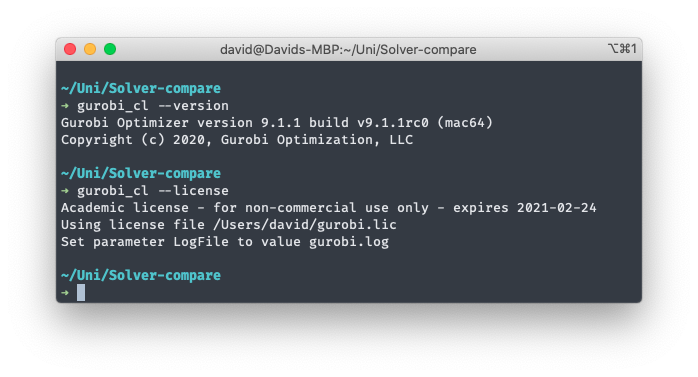
\includegraphics[width=0.6\textwidth]{images/gurobi_license.png}
	\caption{Primer izpisa ukazov za podatke o verziji in licenci po uspešni namestitvi \textit{Gurobi optimizerja} na macOS.}
	\label{img:gurobi_license}
\end{figure}
CLI orodje podpira 14 formatov za podajanje optimizacijskega modela in drugih pomožnih podatkov~\cite{GurobiFormats:2020}. V nadaljevanju bomo uporabljali dva: LP in MPS format. LP format je namenjen za boljšo berljivost iz strani človeka, medtem ko je MPS format najstarejši in najpogosteje uporabljen za shranjevanje matematičnih programskih modelov. MPS format je veliko strožji kar se tiče zapisa (fiksni začetni stolpci za vrednosti ipd.), zato ga bomo le uporabili pri testnih primerih.

\subsection{Reševanje ILP problemov z Gurobi optimizer}

Za boljši vploged v orodje, si bomo v nadaljevanju ogledali enostaven primer optimizacijskega problema in kako se le ta reši s pomčjo Gurobi optimizerja. Predstavljen primer je prilagojena verzija primera v vodiču za hiter zagon~\cite{GurobiQuickstart:2020}. 

\subsubsection{Opis problema}
V času pisanja poročila je blizu konec koledarskega leta. \textit{United States Mint} (ustanova, ki proizvaja ameriške kovance), ima še nekaj neporabljene zaloge materialov za proizvodnjo kovancev. Predpostavimo, da si želijo porabiti vso preteklo zalogo, preden se lotijo nabave materialov za serijo kovancev novo leto. Ustanova proizvaja šest različnih kovancev, sestava katerih pa je podana v tabeli~\ref{tab:us_coins}. Ustanova sedaj želi proizvesti takšne tipe kovancev, da bo njihova skupna vrednost največja. Kakšna naj bo količina vsakega proizvedenega kovanca, če imamo podano zalogo vsakega materiala?
\begin{table}[hb]
	\centering
	\caption{Vsebnost materialov v ameriških kovancih glede na US Mint specifikacijo~\cite{USMintCoins:2019}}.
	\label{tab:us_coins}
	\begin{tabular}{r r r r r r r}
	 & \textbf{Cent} & \textbf{Nickel} & \textbf{Dime} & \textbf{Quarter} & \textbf{Half} & \textbf{Dollar} \\
	 \hline
	Baker \texttt{(Cu)} & $0.0625$g & $3.7500$g & $2.0791$g & $5.1977$g & $10.3954$g & $7.1685$g \\
	Nikelj \texttt{(Ni)} & & $1.2500$g & $0.1889$g & $0.4723$g & $0.9446$g & $0.1620$g \\
	Cink \texttt{(Zn)} & $2.4375$g & & & & & $0.4860$g \\
	Mangan \texttt{(Mn)} & & & & & & $0.2835$g \\
	\hline	
	Skupaj & $2.5$g & $5.0$g & $2.268$g & $5.670$g & $11.340$g & $8.1$g \\
	\end{tabular}
\end{table}

\subsubsection{Priprava vhodnih datotek}
Za rešitev problema potrebujemo izvesti 3 korake:
\begin{enumerate}
\item Določitev odločitvenih spremenljivk
\item Določitev odločitvene funkcije (v tem primeru linearne)
\item Določitev omejitev
\end{enumerate}
Odločitvene spremenljivke so dokaj jasne: zanima nas količina vsakega kovanca, ki ga naj proizvedemo. Ker smo programerji in za lepšo nazornost jim bomo podali opisna imena, za matematike pa še vektorske spremenljivke. Spremenljivke torej poimenujemo \textit{Cents}, \textit{Nickels}, \textit{Dimes}, \textit{Quarters}, \textit{Halves}, \textit{Dollars} (oziroma $x_1$, $x_2$ ... $x_6$). Vpeljimo pa še imena spremenljivk za porabljeno količino materialov \textit{Cu}, \textit{Ni}, \textit{Zn}, \textit{Mn} ($y_1$, $y_2$, $y_3$ in $y_4$). Te spremenljivke so določene in predstavljajo material, ki je na zalogi. Za zalogo bomo predpostavili 1000g bakra in po 50g vsakega ostalega materiala.
Formalen matematični zapis modela (ki ga maksimiziramo) se glasi:
\begin{equation}
	f(x) = 0.01 x_1 + 0.05 x_2 + 0.1 x_3, + 0.25 x_4 + 0.5 x_5 + 1x_6
\end{equation}
pri čemer so $x_n$ količine proizvedenih kovancev, koeficienti pred njimi pa predstavljajo vrednost posameznega kovanca. Omejitve so sledeče:
\begin{equation}
\begin{aligned}
0.0625 x_1 + 3.7500 x_2 + 2.0791 x_3 + 5.1977 x_4 + 10.3954 x_5 + 7.1685 x_6 \leq 1000 \\
1.2500 x_2 + 0.1889 x_3 + 0.4723 x_4 + 0.9446 x_5 + 0.1620 x_6 \leq 50 \\
2.4375 x_1 + 0.4860 x_6 \leq 50 \\
0.2835 x_6 \leq 50 \\
x_1, x_2, x_3, x_4, x_5, x_6 \in \mathbb{N}
\end{aligned}
\end{equation}
Skratka količina porabljenega materiala ne sme presegati zaloge, prav tako pa ne moremo proizvesti manj kot celoto kovanca (celoštevilska omejitev). Isto omejitev lahko zapišemo na programerski način (prej omenjene opisne spremenljivke) in LP format zapisa (glej kodo~\ref{code:coins_lp}). Slednje nam predstavlja enega izmed možnih vhodov v Gurobi optimizer.

\lstinputlisting[language={}, caption=Primer LP formata za problem proizvodnje kovancev,label=code:coins_lp,firstline=5]{code/coins.lp}

LP format ima nekaj posebnosti. V podanem primeru imamo štiri sekcije (\textit{Maximize}, \textit{Subject to}, \textit{Bounds}, \textit{Integers}), ki si morajo vedno slediti v tem vrstnem redu. Sekcij je lahko več in tudi znotraj sekcij se lahko pojavi  več scenarijev. Vse to je opisano v navodilih za uporabo\footnote{Navodila za LP format v Gurobi \url{https://www.gurobi.com/documentation/9.1/refman/lp_format.html\# format:LP}.}. Druga posebnost je zapis vrednosti (spremenljivk, konstant, operatorjev ...). Te morajo biti ločene s presledki oziroma novimi vrsticami. Tako je \texttt{+ 0.1x} napačen zapis. Pravilno je  \texttt{+ 0.1 x}. Tretje splošno pravilo je, da se spremenljivke vedno pišejo na levi in konstante na desni (primer tega je v sekciji \textit{Subject to}). Na koncu pa naj še omenimo, da je po privzetem spodnja meja enaka 0, razen če je eksplicitno zapisana. Zapis \texttt{Cu <= 1000} je v resnici \texttt{0 <= Cu <= 1000}. To pomeni, da Gurobi po privzetem vsako spremenljivko omeji na nenegativna števila.

\subsubsection{Zagon in rešitve}

Najenostavnejši način uporabe Gurobi, kadar imamo podan model v datoteki, je preko ukazne vrstice. Z ukazom \texttt{gurobi\_cl \textless model.lp\textgreater} lahko poženemo orodje in se problem prične reševati. Kot rešitev imamo na standardnem izhodu podano samo vrednost cenitvene funkcije, če želimo videti še vrednosti posameznih spremenljivk, je potrebno dodati parameter \texttt{ResultFile=<izhod.sol>}. Celoten ukaz je torej: \\
\texttt{gurobi\_cl ResultFile=code/coins.sol code/coins.lp}\\
Izpis ukaza je viden na sliki~\ref{img:coins_stdout}, izhodna datoteka z rešitvami pa v kodi~\ref{code:coins_sol}.

\begin{figure}[htpb] \centering
	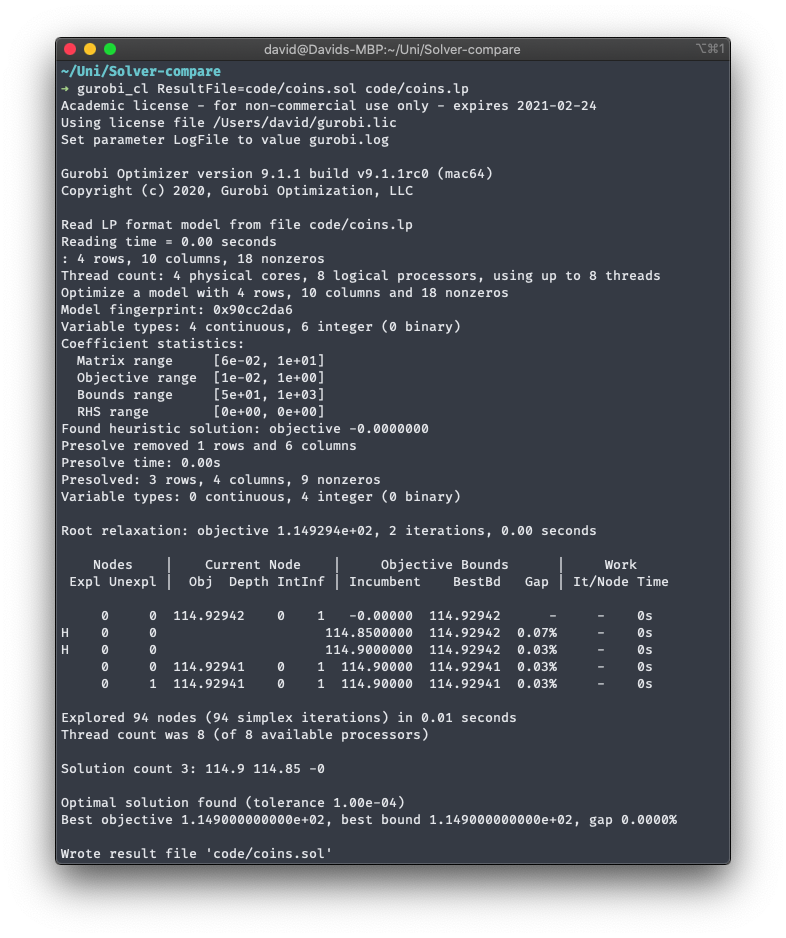
\includegraphics[width=0.6\textwidth]{images/gurobi-run_coins.png}
	\caption{Primer izpisa na standardni izhod pri reševanju problema s kovanci.}
	\label{img:coins_stdout}
\end{figure}

\lstinputlisting[language={}, caption=Generirana datoteka z reštivami za problem kovancev,label=code:coins_sol]{code/coins.sol}

Na standardnem izhodu ukaza lahko vidimo nekaj podatkov o problemu, vidimo da se je problem reševal v 8 nitih in da je potreboval 94 Simplex iteracij za doseženo rešitev \$114.9. V izhodni datoteki z rešitvami pa se nahajajo še količine posameznih kovancev: 4 \textit{Dimes}, 50 \textit{Quarters} in 102 \textit{Dollars}.

Obstaja tudi \textit{Gurobi Interactive Shell}, ki temelji na \textit{Python Shell}. Potek ukazov je zelo podoben programiranju v Python, omogoča pa hitrejše spreminjanje modela in zaganjanje v primerjavi z ročnim spreminjanjem vhodne datoteke in vnovičnega poganjanja ukazov. Bolj podroben opis je na voljo v uradni dokumentaciji ali v hitrem vodiču~\cite{GurobiQuickstart:2020}.

\subsection{Uporaba s Python}
Gurobi ima na voljo tudi vmensik za Python. Slednjega lahko namestimo na tri načine: preko \texttt{pip}, ročno ali pa uproabimo \texttt{Anaconda}. Ne glede na način, ki ga izberemo bo še vedno potrebna pridobitev in namestitev veljavne licence, kot smo opisali v enemu izmed prejšnjih poglavjih. Za potrebe te naloge smo se odločili za namestitev v Python virtualno okolje in uporabo \texttt{pip}. Paket se imenuje \texttt{gurobipy} in v času pisanja naloge (še) ni bil dostopen v javnem PyPi strežniku. Zato se za namestitev uporabi njihov privaten strežnik in ukaz:  \\
\texttt{python3 -m pip install -i https://pypi.gurobi.com gurobipy} \\
Ročna namestitev se izvede s pomočjo \texttt{setup.py}, ki se nahaja znotraj mape kamor smo namestili Gurobi med pridobivanjem licence. Pri obeh omenjenih načinih namestitve je potrebno paziti na kompatibilno verzijo Python (podprte so 2.7 in 3.6 - 3.9 in le 64-bitne različice). Zadnja možnost pa je uporaba Anaconde\footnote{Anaconda je distribucija Pythona dosegljiva na \url{https://www.anaconda.com/}} \\
\texttt{conda config --add channels https://conda.anaconda.org/gurobi} \\
\texttt{conda install gurobi} 

Namestitev se lahko preveri tudi s pomočjo \texttt{Jupyter notebook}, ki bi moral biti priložen temu poročilu (nahaja se v  \texttt{code/Gurobi-demo.ipynb}). V kolikor si pa bralec želi igrati s tem Jupyter zvezkom, pa je na voljo tudi \texttt{requirements.txt}. V splošnem za zvezek potrebujete \texttt{numpy}, \texttt{scipy} in \texttt{gurobipy} (iz privatnega strežnika), vse drugega so odvisnosti teh paketov. Primer ukazov za macOS/Linux, ki pripravijo okolje in odprejo zvezek za urejanje: \\
\texttt{python3 -m venv genv} \\
\texttt{source genv/bin/activate} \\
\texttt{python3 -m pip install -r requirements.txt} \\
\texttt{jupyter notebook code/Gurobi-demo.ipynb} \\
Bralec, ki si ne želi urejati zvezek, si lahkotudi  ogleda statičen zvezek na Github repozitoriju kjer se nahaja to poročilo\footnote{Povezava do Jupyter zvezka \url{https://github.com/rubinda/gurobi-vs-matlab/blob/main/code/Gurobi-demo.ipynb}}. Hiter povzetek uporabe Gurobi v Python skupaj z LP datotekami je viden v kodi~\ref{code:gurobipy}.

\begin{lstlisting}[language=Python,caption=Primer uporabe LP formatov in gurobipy,label=code:gurobipy]
import gurobipy as gp

m = gp.read('coins.lp') # preberi model
m.optimize() # optimiziraj

# izpisi rezultate
for v in m.getVars(): 
    print(f'{v.varName}={v.x}')
print(f'vrednost: {m.objVal}')
\end{lstlisting}

\subsection{Uporaba z MATLAB}
\label{gurobi_matlab}

Enako kot pri Python paketu je treba najprej namestiti knjižnice in pridobiti veljavo licenco (opisano v poglavju~\ref{gurobi_install}). Za delo z MATLAB so pri Gurobi pripravili skripto, ki nam pomaga pri namestitvi vmesnika. Ta skripta (\texttt{gurobi\_setup.m}) se nahaja v mapi \texttt{matlab} v direktoriju kamor smo namestili Gurobi. Privzeta lokacija (verzija 9.1.1) na macOS je \texttt{/Library/gurobi911/\-mac64/matlab} in na Windows \texttt{c:\textbackslash gurobi911\textbackslash win64\textbackslash matlab}. Celoten ukaz namestitve na macOS (klican znotraj MATLAB-a) je potemtakem: \\
\texttt{cd /Library/gurobi911/mac64/matlab} \\
\texttt{gurobi\_setup} \\
 V kolikor se pojavi kakšna napaka je dobro najprej preveriti ali upoštevamo kompatibilnost, saj Gurobi podpira le 64-bitno različico MATLAB-a. Ob uspešeni namestitvi bi se moral pojaviti napis podoben temu na sliki~\ref{img:gurobi_matlab_install}.
\begin{figure}[hbpt]
	\centering
	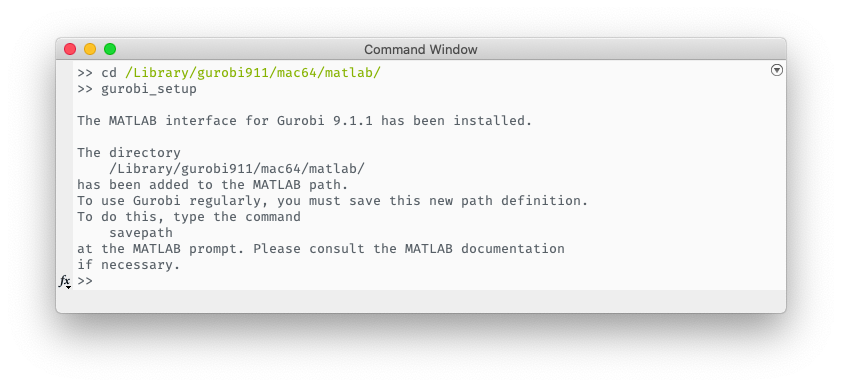
\includegraphics[width=0.6\textwidth]{images/gurobi_matlab_install.png}
	\caption{Izpis skripte po uspešni namestivi Gurobi rutin v MATLAB na macOS.}
	\label{img:gurobi_matlab_install}
\end{figure}

Pokažimo osnovno uporabo na enakem problemu kot pri Python. V kolikor niste sledili Python zvezku, je problem sledeč:
\begin{equation}
\begin{aligned}
\textbf{maksimiziraj} \hspace{3mm} x + y + 2z  \\
\textbf{ob omejitvah} \hspace{2mm} x + 2y + 3z \leq 4\\
x + y \geq 1 \\
x, y, z \text{ so binarne}
\end{aligned}
\end{equation}

V MATLAB si lahko pripravimo skript, ki s pomočjo Gurobi opiše problem, ga shrani kot LP format in požene optimizacijo (koda~\ref{code:gurobi_matlab_script}).

\lstinputlisting[language=Matlab,caption=Reševanje osnovnega problema v MATLAB s pomočjo Gurobi,label=code:gurobi_matlab_script]{code/gurobi_demo.m}

Standardni izhod ob klicanju skripte je prikazan na sliki~\ref{img:gurobi_matlab_demo_run}. Glaven ukaz je \texttt{gurobi(model, params)}, kjer podamo podatke o problemu in pa parametre za optimizacijo. Vse parametre in več o uporabi si bralec lahko prebere v uradni dokumentaciji~\footnote{Uradna Gurobi dokumentacija za MATLAB vmesnik je dostopna na \url{https://www.gurobi.com/documentation/9.1/refman/matlab\_api\_overview.html\#matlab:MATLAB}}. Za boljšo predstavo pa je na voljo tudi več primerov uporabe, ki se nahajajo v mapi namestitve Gurobi (torej \texttt{\textless direktorij namestitve\textgreater /examples/matlab}).
\begin{figure}[hbpt]
	\centering
	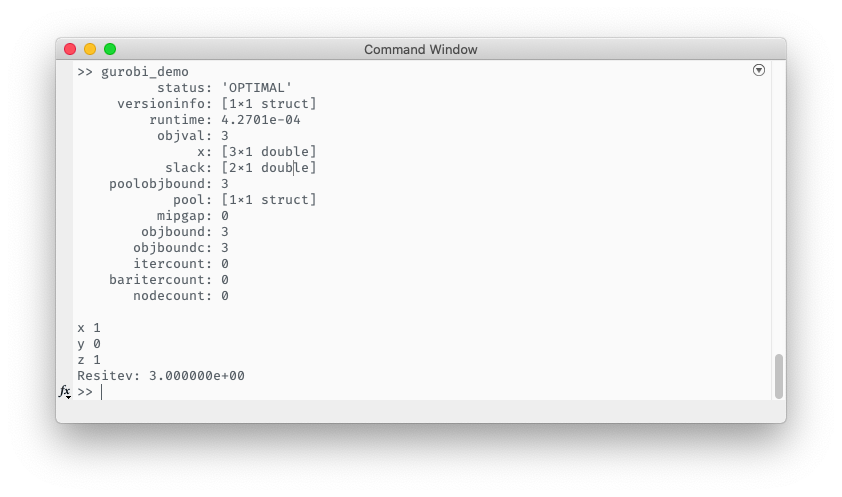
\includegraphics[width=0.6\textwidth]{images/gurobi_matlab_demo_run.png}
	\caption{Izpis rešitve ob uporabi \texttt{gurobi\_demo} skripte.}
	\label{img:gurobi_matlab_demo_run}
\end{figure}

Poglejmo si zdaj še primer, kadar želimo uporabiti obsotejčo LP datoteko preko MATLAB vmesnika. Gurobi ponuja med drugim tudi funkcijo, ki to omogoča na zelo enostaven način (glej kodo~\ref{code:gurobi_matlab_demo_file} in sliko~\ref{img:matlab_gurobi_demo_file}).

\lstinputlisting[language=Matlab,caption=Primer reševanja LP problema s Gurobi MATLAB vmesnikom,label=code:gurobi_matlab_demo_file]{code/gurobi_demo_file.m}
\begin{figure}[htpb]
	\centering
	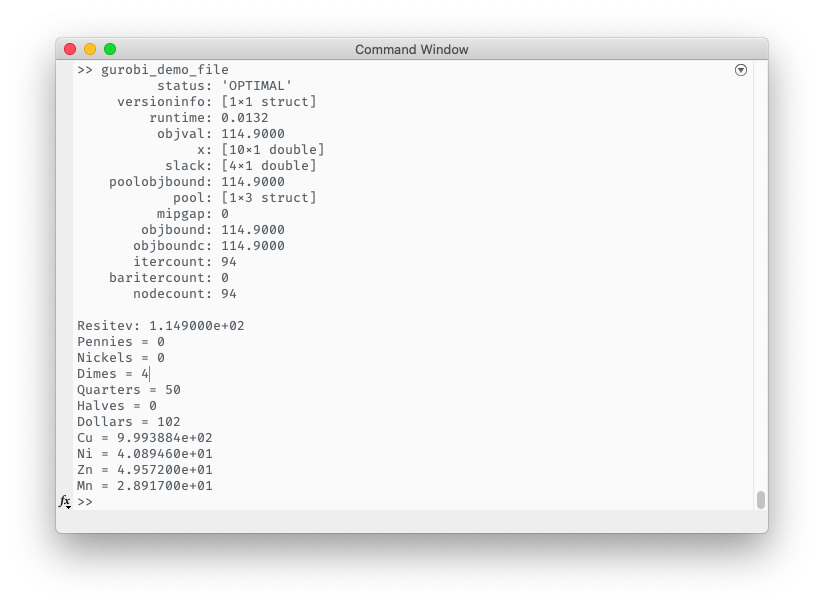
\includegraphics[width=0.6\textwidth]{images/gurobi_matlab_demo_file.png}
	\caption{Standardni izhod pri zagou \texttt{gurobi\_demo\_file.m} skripte.}
	\label{img:matlab_gurobi_demo_file}
\end{figure}


\section{Testna zbirka}
\label{benchmark_data}
Testna zbirka MIPLIB2017 je nastala zaradi potrebe raziskovalcev po primerih MIP (angl. \textit{mixed integer programs}) iz realnega sveta. V tem delu smo sicer želeli primerjati le celoštevilske probleme, vendar smo se zaradi enostavnejše primerjave odločili, da uporabimo kar nekaj primerov iz celotne testne zbirke, ki jo sestavljajo tudi mešani primeri (poleg celoštevilskih vsebujejo tudi zvezne spremenljivke). Drugi razlog za izbiro te zbirke je tudi dejstvo, da se je uveljavila kot standardni performančni test, v katerega so prispevali tudi vsi večji ponudniki optimizacijske programske opreme (Gurobi, CPLEX, Fico, MOSEK ...)\textit{Benchmark set} sestavlja 240 problemov, ki so zaradi praktičnih razlogov izbrani kot primeri z dobro numerično stabilnostjo in dobro rešljivostjo. \textit{Collection set} pa vsebuje še veliko več problemov, med katerimi so tudi še nerešeni. ~\cite{Miplib:2017}.

Vsak izmed primerov je kategoriziran med težke ali lahke primere, podan pa ima tudi kratek opis o parametrih, omejitvah ipd. Na sliki~\ref{img:miplib_sample_set} vidimo izsek o predstavitvi enega izmed primerov. Tašne predstavitve teh problemov so dostopne preko spletne strani \url{http://miplib.zib.de/tag_benchmark.html}.
\begin{figure}[htpb]
	\centering
	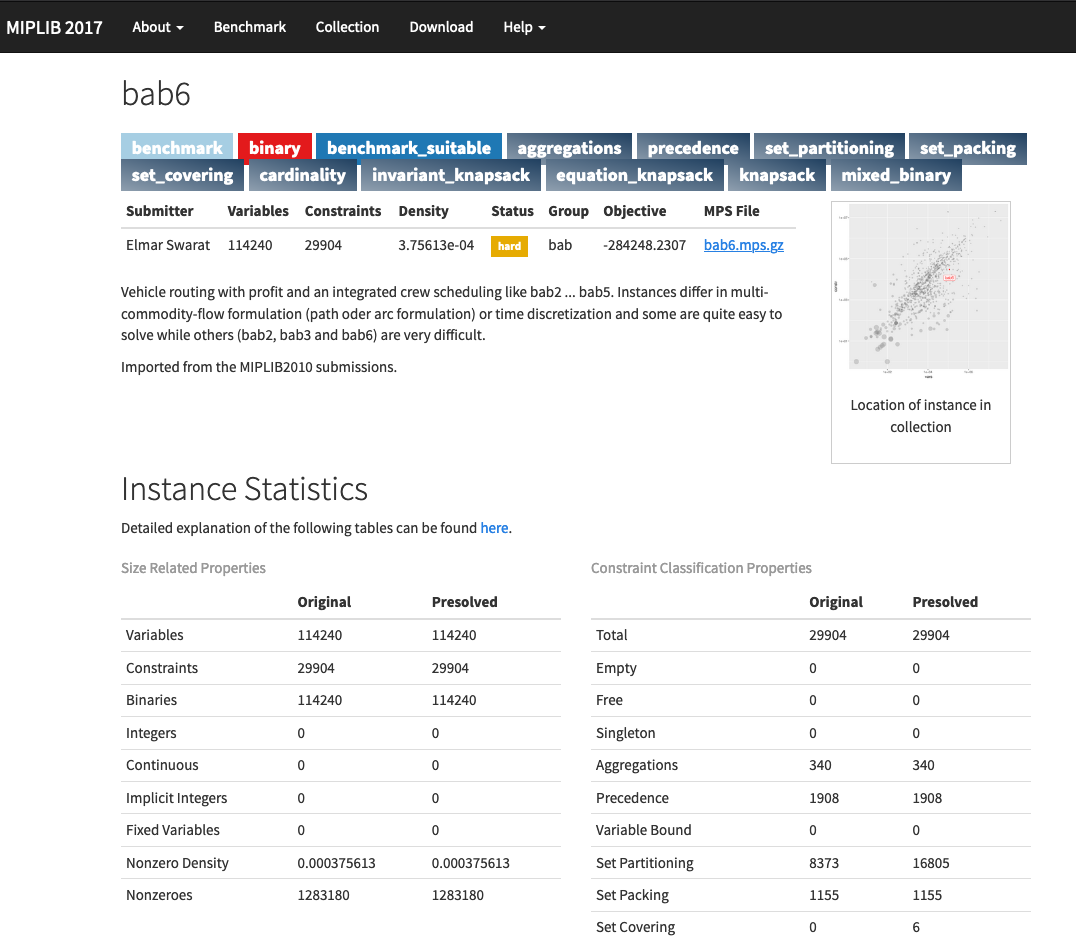
\includegraphics[width=0.8\textwidth]{images/miplib_sample_set.png}
	\caption{Predstavitev problema \texttt{bab6} na MIPLIB2017 spletni strani. \footnotesize Vir: \url{http://miplib.zib.de/instance_details_bab6.html}}
	\label{img:miplib_sample_set}
\end{figure}

Zaradi omejitev strojne opreme (in posledično časovne) smo iz zbirke izbrali nekaj problemov, za katere smo preverili, da so rešljivi v relativno kratkem času. Težava s to testno zbirko je, da predvideva reševanje od precej enostavnih do relativno težkih problemov, ki se rešujejo s pomočjo distribuiranih sistemov. Primer takšnega problema, ki se sicer šteje med lažje, je \texttt{50v-10} (opis na  \url{http://miplib.zib.de/instance_details_50v-10.html}). Za slednjega navajajo, da so rešitev našli s pomočjo 2.000 jedrnega super računalnika, žal pa sami do takšne računske zmogljivosti nimamo dostopa.

\section{Primerjava Gurobi in Matlab}
Celotno testiranje smo izvedli v okolju MATLAB. Izbrali smo 10 problemov iz testne zbirke in vsakega trikrat poskusili rešiti s pomočjo MATLAB-ovega \texttt{intlinprog} in pa s Gurobi preko MATLAB vmesnika. Pri Gurobi smo preverili tudi hitrost reševanja ob uporabi 1, 2, 4 ali 8 jeder (omejitev računalnika). Skripta, ki nam to omogoča se imenuje \texttt{bench\_gurobi.m} in bi morala biti priložena temu poročilu. Za njeno uporabo je potreben MATLAB (64-bitna različina z nameščenim \textit{optimization toolbox}) in Gurobi MATLAB vmesnik z veljavno licenco (glej poglavje~\ref{gurobi_install} glede pridobitve licence in poglavje~\ref{gurobi_matlab} za uporabo Gurobi z MATLAB).

\subsection{Testno okolje}
Testiranje se je izvajalo na prenosnem računalniku v operacijskem sistemu macOS. Procesor je 4-jedrni (8 niti) Intel Core i7 4700HQ, na voljo pa je imel 8GB delovnega pomnilnika (glej sliko~\ref{img:davids_mbp}). Verzija MATLAB je bila R2020b (9.9.0.1467703) 64-bitna različia iz 26. avgusta 2020, verzija Gurobi pa 9.1.1 build v9.1.1rc0 (mac64). Med posameznimi zagoni so tekli le najnujnejši procesi (torej ali MATLAB ali okno ukazne vrstice z Gurobi), prav tako pa je bil prenosnik priključen v napajanje in ni izvajal kakršnihkoli drugih opravil.

\begin{figure}[htpb]
	\centering
	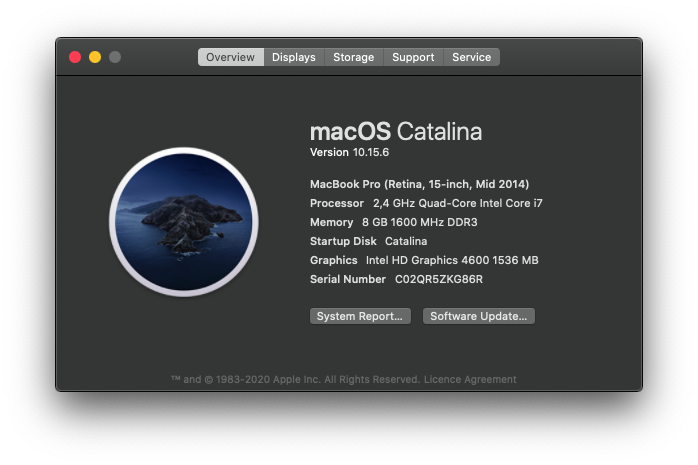
\includegraphics[width=0.7\textwidth]{images/davids-mbp.png}
	\caption{Podaki računalnika, na katerem se je izvajalo performančno testiranje}
	\label{img:davids_mbp}
\end{figure}

\subsection{Performančni rezultati}
Izrisi grafe za zagone in resene probleme

\section{Zaključek}
Povzemi kaj smo naredili, kaj smo ugotovili.

\appendix
\appendixpage
\section{\label{app-res}Podrobni rezultati poskusov}

Če je rezultatov v smislu tabel ali pa grafov v nalogi mnogo,
predstavi v osnovnem besedilu samo glavne, podroben prikaz
rezultatov pa lahko predstaviš v prilogi. V glavnem besedilu ne
pozabi navesti, da so podrobni rezultati podani v prilogi.

\section{Programska koda}

Za domače naloge bo tipično potrebno kaj sprogramirati. Če ne bo od
vas zahtevano, da kodo oddate posebej, to vključite v prilogo. Čisto
za okus sem tu postavil nekaj kode, ki uporablja Orange
(\url{http://www.biolab.si/orange}) in razvrščanje v skupine.


\bibliographystyle{acm}
\bibliography{bibliography.bib}

\end{document}
